% Shared content: each frame is one static PDF page in both languages.
% English first, Chinese second in every \bi. Geometries and equations are shared.
\documentclass[aspectratio=169,11pt]{beamer}
\usepackage{fix-cm}
\usepackage[fontset=fandol]{ctex}
\xeCJKsetup{CJKglue=\hskip 0pt}
\usepackage{fontspec}
\setsansfont{texgyreheros}[Extension=.otf,UprightFont=*-regular,
 BoldFont=*-bold,ItalicFont=*-italic,BoldItalicFont=*-bolditalic]
\usepackage{amsmath,amssymb,booktabs,array,tikz,pgfplots}
\usetikzlibrary{arrows.meta,positioning,calc,shapes.geometric}
\pgfplotsset{compat=1.18}
\definecolor{Navy}{HTML}{17334D}
\definecolor{Ink}{HTML}{263C4C}
\definecolor{Muted}{HTML}{617789}
\definecolor{Teal}{HTML}{007E87}
\definecolor{Blue}{HTML}{326FC0}
\definecolor{Amber}{HTML}{BA7216}
\definecolor{Purple}{HTML}{8557AD}
\definecolor{Red}{HTML}{B63E4A}
\definecolor{Road}{HTML}{EEF1F4}
\definecolor{Rule}{HTML}{D7E0E7}
\setbeamercolor{normal text}{fg=Ink,bg=white}
\setbeamercolor{frametitle}{fg=Navy}
\setbeamercolor{structure}{fg=Teal}
\setbeamercolor{alerted text}{fg=Red}
\setbeamerfont{frametitle}{size=\Large,series=\bfseries}
\setbeamersize{text margin left=8mm,text margin right=8mm}
\setbeamertemplate{navigation symbols}{}
\setbeamertemplate{frametitle}{\vbox to 12mm{\vfil\hbox{\strut\insertframetitle}\vskip2mm}}
\setbeamertemplate{footline}{\hspace{8mm}\textcolor{Muted}{\fontsize{6.5}{8}\selectfont\bi{DECISION-BARRIER FRAMEWORK}{决策屏障框架}}\hfill\textcolor{Muted}{\fontsize{7}{8}\selectfont\insertframenumber\,/\,18}\hspace{8mm}\vspace{2.5mm}}
\setbeamertemplate{itemize item}{\color{Teal}\small\textbullet}
\setlength{\parskip}{2mm}
\newcommand{\bi}[2]{\ifChinese#2\else#1\fi}
\newcommand{\lead}[2]{\par{\color{Teal}\large\bi{#1}{#2}\par}\vspace{1mm}}
\newcommand{\srcnote}[2]{\par{\color{Muted}\scriptsize\bi{#1}{#2}\par}}
\newcommand{\warn}[2]{\par{\color{Red}\small\bi{#1}{#2}\par}}
\newcommand{\sect}[2]{\par{\color{Navy}\bfseries\bi{#1}{#2}\par}}
\newcommand{\gap}{\par\vspace{2mm}}
\newcolumntype{P}[1]{>{\raggedright\arraybackslash}p{#1}}
\tikzset{>=Latex,
 every node/.style={font=\small,text=Ink},
 arr/.style={-{Latex[length=2mm]},thick,draw=Muted},
 lane/.style={-{Latex[length=2mm]},line width=1.1pt},
 dot/.style={circle,fill=white,draw=Red,thick,inner sep=1.3pt},
 stage/.style={draw=Rule,fill=white,minimum height=11mm,align=center,text width=26mm,font=\small},
 graph/.style={circle,draw=Teal,thick,fill=white,minimum size=9mm,font=\scriptsize},
 tag/.style={font=\scriptsize,fill=white,inner sep=1.5pt},
 }
% Car rectangles are entirely editable in TikZ. #1 x, #2 y, #3 color,
% #4 heading rotation in degrees, #5 label. Local +x is forward.
\newcommand{\car}[5]{\begin{scope}[shift={(#1,#2)},rotate=#4]
 \filldraw[fill=#3,draw=white,line width=.6pt,rounded corners=.035cm](-.25,-.12) rectangle (.25,.12);
 \draw[white,line width=.8pt](.13,-.075)--(.13,.075);
 \end{scope}\node[font=\scriptsize,text=white]at(#1,#2){#5};}
\newcommand{\ghostcar}[4]{\begin{scope}[shift={(#1,#2)},rotate=#4]
 \draw[draw=#3,line width=.8pt,rounded corners=.035cm](-.25,-.12) rectangle (.25,.12);
 \end{scope}}
% Lane IDs mean travel direction: NS is north to south (right-hand traffic).
% EW lies at y=.38; WE lies at y=-.38. c1..c4 match all graphs/matrices.
\newcommand{\roadbase}[1]{
 \fill[Road](-.75,-2.05)rectangle(.75,2.05);
 \ifnum#1=1\fill[Road](-2.7,.03)rectangle(2.7,.73);\else\fill[Road](-2.7,-.75)rectangle(2.7,.75);\fi
 \draw[white,line width=1pt,dashed](0,-2.05)--(0,2.05);
 \ifnum#1=2\draw[white,line width=1pt,dashed](-2.7,0)--(2.7,0);\fi
 \draw[lane,Teal](-.38,1.95)--(-.38,-1.95);
 \draw[lane,Blue](.38,-1.95)--(.38,1.95);
 \draw[lane,Amber](2.6,.38)--(-2.6,.38);
 \ifnum#1=2\draw[lane,Purple](-2.6,-.38)--(2.6,-.38);\fi
 \node[tag,text=Teal,anchor=east]at(-.5,1.8){NS};
 \node[tag,text=Blue,anchor=west]at(.5,-1.8){SN};
 \node[tag,text=Amber,anchor=south]at(2.4,.55){EW};
 \ifnum#1=2\node[tag,text=Purple,anchor=north]at(-2.4,-.55){WE};\fi
}
\newcommand{\conflicts}[1]{
 \node[dot]at(-.38,.38){};\node[tag,anchor=south east]at(-.43,.47){$c_1$};
 \node[dot]at(.38,.38){};\node[tag,anchor=south west]at(.43,.47){$c_2$};
 \ifnum#1=2
 \node[dot]at(-.38,-.38){};\node[tag,anchor=north east]at(-.43,-.47){$c_3$};
 \node[dot]at(.38,-.38){};\node[tag,anchor=north west]at(.43,-.47){$c_4$};\fi
}
\newcommand{\graphA}{
 \node[graph,draw=Teal](ns)at(0,1.1){NS};
 \node[graph,draw=Blue](sn)at(0,-1.1){SN};
 \node[graph,draw=Amber](ew)at(2.3,0){EW};
 \draw[thick,Teal](ns)--node[tag]{$c_1$}(ew);
 \draw[thick,Blue](sn)--node[tag]{$c_2$}(ew);
}
\newcommand{\graphB}{
 \node[graph,draw=Teal](ns)at(0,1.1){NS};
 \node[graph,draw=Blue](sn)at(0,-1.1){SN};
 \node[graph,draw=Amber](ew)at(2.4,1.1){EW};
 \node[graph,draw=Purple](we)at(2.4,-1.1){WE};
 \draw[thick,Teal](ns)--node[tag]{$c_1$}(ew);
 \draw[thick,Blue](sn)--node[tag]{$c_4$}(we);
 \draw[thick,Amber](sn)--node[tag,pos=.28]{$c_2$}(ew);
 \draw[thick,Purple](ns)--node[tag,pos=.28]{$c_3$}(we);
}
\hypersetup{pdftitle={\ifChinese 决策屏障框架\else Decision-Barrier Framework\fi},pdfsubject={Idea Note 2026-07-08; method explanation and proposed experiments},colorlinks=true,urlcolor=Teal}

\begin{document}

% 01 -----------------------------------------------------------------
\begin{frame}[t]
\vspace{5mm}
\begin{columns}[T,onlytextwidth]
\column{.57\textwidth}
{\color{Teal}\small\bi{IDEA NOTE / 2026-07-08}{研究构想 / 2026-07-08}\par}
\vspace{5mm}
{\color{Navy}\LARGE\bfseries\bi{Decision-Barrier\\Framework}{决策屏障框架}\par}
\vspace{4mm}
{\large\bi{Barrier-Based Platoon Control for Autonomous Intersection Management}{面向自动驾驶交叉口管理的\\基于屏障的车队控制}\par}
\vspace{5mm}
\lead{How are crossing order and speed correction connected?}{通行顺序如何转化为车辆控制修正？}
\srcnote{Method explanation and proposed experiments}{方法讲解与未来实验设计}
\column{.40\textwidth}
\centering
\begin{tikzpicture}[scale=.84,transform shape]
 \roadbase{1}\conflicts{1}
 \car{-.38}{1.25}{Teal}{-90}{A}
 \car{1.85}{.38}{Amber}{180}{B}
 \draw[Red,densely dashed,rounded corners](-.85,-.05)rectangle(.85,.85);
 \node[font=\small,align=center]at(0,-2.55){$A\prec B$\\\bi{Order first; correction follows}{先定顺序，再计算修正}};
\end{tikzpicture}\par
\end{columns}
\end{frame}

% 02 -----------------------------------------------------------------
\begin{frame}[t]{\bi{Two layers, one feedback loop}{两层结构与一个反馈循环}}
\lead{The decision layer chooses who yields}{决策层确定谁先行、谁让行}
\centering
\begin{tikzpicture}[x=1cm,y=1cm]
 \node[stage](s)at(1.5,0){\bi{Observe\\state + path}{观测状态\\位置与速度\\车道与路径}};
 \node[stage](f)at(5.0,0){\bi{Filter\\relevant conflicts}{筛选车辆\\窗口与路径}};
 \node[stage,draw=Teal](d)at(8.5,0){\bi{Decision layer\\crossing order}{决策层\\确定通行顺序}};
 \node[stage,draw=Amber](b)at(12,0){\bi{Barrier layer\\margin + correction}{屏障层\\裕度与控制修正}};
 \draw[arr](s)--(f);\draw[arr](f)--(d);\draw[arr](d)--(b);
 \node[stage](n)at(5,-1.85){\bi{Nominal headway\\control}{名义控制\\车头时距}};
 \node[circle,draw=Teal,thick,minimum size=8mm](sum)at(8.5,-1.85){$+$};
 \node[stage](e)at(12,-1.85){\bi{Execute one sample\\update the state}{执行采样周期\\更新车辆状态}};
 \draw[arr](n)--(sum);\draw[arr](b.south)--++(0,-.45)-|(sum.north);
 \draw[arr](sum)--node[above,font=\scriptsize]{$u_i$}(e);
 \draw[arr](e.south)--++(0,-.65)-|(s.south);
 \node[tag]at(5,-3.05){\bi{New observation at the next sample}{下一采样时刻重新观测}};
\end{tikzpicture}\par
\vspace{2mm}
\begin{columns}[T,onlytextwidth]
\column{.48\textwidth}\sect{Spatial filter}{空间筛选}
\small\bi{Inside the approach window and sharing a conflict.}{进入接近窗口，且路径具有冲突关系。}
\column{.48\textwidth}\sect{Time-margin test}{时间裕度判断}
\small\bi{Apply the activation threshold only to these pairs.}{只对相关车辆对判断屏障是否激活。}
\end{columns}
\end{frame}

% 03 -----------------------------------------------------------------
\begin{frame}[t]{\bi{Arrival time adds the missing speed information}{到达时间补充了距离无法表达的速度信息}}
\begin{columns}[T,onlytextwidth]
\column{.53\textwidth}
\begin{tikzpicture}[x=1cm,y=1cm]
 \fill[Road](0,-.28)rectangle(5.8,.28);
 \fill[Road](0,-1.98)rectangle(5.8,-1.42);
 \car{.5}{0}{Teal}{0}{A}\car{.5}{-1.7}{Amber}{0}{B}
 \draw[lane,Teal](1,0)--(5.1,0);
 \draw[lane,Amber](1,-1.7)--(5.1,-1.7);
 \draw[dashed,Red](5.3,.5)--(5.3,-2.2);
 \node[tag,anchor=west]at(5.35,-.8){$c_m$};
 \draw[<->,Muted](.5,.55)--node[tag]{$d_A=30\,\mathrm m$}(5.3,.55);
 \draw[<->,Muted](.5,-2.2)--node[tag]{$d_B=30\,\mathrm m$}(5.3,-2.2);
 \node[tag]at(2.7,-.5){$v_A=10\,\mathrm{m/s}$};
 \node[tag]at(2.7,-1.15){$v_B=6\,\mathrm{m/s}$};
 \node[font=\small,align=center]at(2.8,-3){\bi{Same distance, different predicted arrivals}{距离相同，预计到达时刻不同}};
\end{tikzpicture}\par
\column{.43\textwidth}
\[
 T_i^m=\frac{d_i^m}{\max(v_i,v_{\min})}
\]
\begin{align*}
 T_A&=\frac{30}{10}=\textcolor{Teal}{3\,\mathrm s},\\[3pt]
 T_B&=\frac{30}{6}=\textcolor{Amber}{5\,\mathrm s}.
\end{align*}
\small\bi{Distance follows the planned path. Prediction assumes the current speed.}{距离沿计划行驶路径测量，到达时间按当前速度外推。}
\gap
\srcnote{Arrival-time estimate is not collision TTC. This example uses speeds above the floor.}{预计到达时间不等于碰撞 TTC；本例速度均高于下限。}
\end{columns}
\end{frame}

% 04 -----------------------------------------------------------------
\begin{frame}[t]{\bi{The decision layer selects a crossing order}{决策层如何选择通行顺序}}
\begin{columns}[T,onlytextwidth]
\column{.46\textwidth}
\sect{Start with arrival time}{先采用到达时间排序}
\[J_i^m=T_i^m,\qquad\mathcal O^m=(A,B,C)\]
\small\bi{A smaller score gives higher priority.}{评分越小，通行优先级越高。}
\gap
\sect{Extensions in the draft}{原文中的扩展评分}
\small
\[J_i^m=\lambda_1T_i^m+\lambda_2Q_{l_i}+\lambda_3P_{l_i}+\lambda_4R_i\]
\bi{$Q$: queue length; $P$: road priority;\\$R$: maneuver priority.}{$Q$：排队长度；$P$：道路优先级；\\$R$：行驶动作优先级。}
\column{.50\textwidth}
\begin{tikzpicture}[x=.72cm,y=1cm]
 \draw[arr](0,0)--(8.4,0)node[below,font=\scriptsize]{$T\ (\mathrm s)$};
 \foreach \x in {0,1,...,7}{\draw[Muted](\x,.06)--(\x,-.06);\node[below,font=\scriptsize]at(\x,-.06){\x};}
 \foreach \x/\n/\c in {3/A/Teal,5/B/Amber,7/C/Blue}{
 \draw[\c,thick](\x,0)--(\x,.75);\node[circle,fill=\c,text=white,minimum size=6mm]at(\x,.9){\n};}
 \node[font=\Large,text=Teal]at(4,-1){$A\prec B\prec C$};
 \node[align=center,text width=5.5cm,font=\small]at(4,-2){\bi{The barrier layer acts on\\the selected order}{屏障层根据选定顺序\\计算让行修正}};
\end{tikzpicture}\par
\end{columns}
\vspace{3mm}
\srcnote{Tie-breaking, order retention, and consistency across conflict points still require explicit implementation rules.}{同分处理、顺序保持与跨冲突点的一致性，仍需补充明确的实现规则。}
\end{frame}

% 05 -----------------------------------------------------------------
\begin{frame}[t]{\bi{Safety margin and activation threshold}{安全裕度与激活阈值}}
\begin{columns}[T,onlytextwidth]
\column{.48\textwidth}\sect{Symmetric separation}{对称时间间隔}
\[h_{ij}^{m,\mathrm{sym}}=|T_i^m-T_j^m|-T_{\mathrm{safe}}\]
\column{.48\textwidth}\sect{After choosing $a\prec b$}{确定 $a\prec b$ 之后}
\[h_{ab}^{m,\mathrm{ord}}=T_b^m-T_a^m-T_{\mathrm{safe}}\]
\end{columns}
\vspace{3mm}
\centering
\begin{tikzpicture}[x=1cm,y=1cm]
 \fill[Red!12](0,0)rectangle(4,.6);
 \fill[Amber!16](4,0)rectangle(8,.6);
 \fill[Teal!12](8,0)rectangle(13.3,.6);
 \draw[arr](0,0)--(13.6,0)node[right]{$h$};
 \draw[Red,thick](4,-.15)--(4,.75);\node[above]at(4,.75){$0$};
 \draw[Amber,thick](8,-.15)--(8,.75);\node[above]at(8,.75){$h_{\mathrm{act}}$};
 \node[align=center,text width=3.5cm,font=\small]at(2,-.75){\bi{Boundary / violation\\$h\leq0$}{边界或违反\\$h\leq0$}};
 \node[align=center,text width=3.5cm,font=\small]at(6,-.75){\bi{Positive, active\\$0<h<h_{\mathrm{act}}$}{裕度为正，屏障激活\\$0<h<h_{\mathrm{act}}$}};
 \node[align=center,text width=4.5cm,font=\small]at(10.6,-.75){\bi{Correction off\\$h\geq h_{\mathrm{act}}$}{关闭屏障修正\\$h\geq h_{\mathrm{act}}$}};
\end{tikzpicture}\par
\vspace{2mm}
\lead{Activation starts before the margin reaches zero}{裕度尚未降到零，屏障就开始干预}
\srcnote{Apply this test only to conflict-relevant vehicles. Ordered and symmetric margins are distinct definitions.}{只对冲突相关车辆进行此判断；有序裕度和对称裕度是两种不同定义。}
\end{frame}

% 06 -----------------------------------------------------------------
\begin{frame}[t]{\bi{Smaller positive margins produce larger corrections}{正裕度越小，屏障修正越强}}
\begin{columns}[T,onlytextwidth]
\column{.44\textwidth}
\sect{Original heuristic expression}{原文中的启发式表达}
\[
 \phi(h)=\begin{cases}-1/h,&h<h_{\mathrm{act}},\\[3pt]0,&h\geq h_{\mathrm{act}}.\end{cases}
\]
\small\bi{On $0<h<h_{\mathrm{act}}$, a smaller margin gives a stronger negative correction.}{在 $0<h<h_{\mathrm{act}}$ 内，裕度越小，负向修正越强。}
\gap
\warn{Undefined at $h=0$; sign reversal for $h<0$.}{在 $h=0$ 处无定义；在 $h<0$ 时符号反转。}
\srcnote{The plotted domain is $h>0$. Threshold is illustrative.}{曲线只绘制 $h>0$ 部分，阈值为示意参数。}
\column{.53\textwidth}
\begin{tikzpicture}
 \begin{axis}[width=7.6cm,height=5cm,xmin=0,xmax=2.3,ymin=-6,ymax=.65,
 axis lines=left,xlabel={$h\ (\mathrm s)$},ylabel={$\phi(h)\ (\mathrm{s}^{-1})$},
 xtick={0,.5,1,1.5,2},ytick={-6,-4,-2,0},tick label style={font=\scriptsize},
 label style={font=\small},grid=major,grid style={Rule!65},clip=false]
 \addplot[Amber,line width=1.5pt,domain=.17:1,samples=80]{-1/x};
 \addplot[Teal,line width=1.5pt,domain=1:2.2]{0};
 \draw[Muted,dashed](axis cs:1,-5.7)--(axis cs:1,.35);
 \addplot[only marks,mark=o,mark options={draw=Amber,fill=white},mark size=2.5pt]coordinates{(1,-1)};
 \addplot[only marks,mark=*,Teal,mark size=2.5pt]coordinates{(1,0)};
 \addplot[only marks,mark=*,Amber,mark size=2.7pt]coordinates{(.5,-2)};
 \node[tag,anchor=west]at(axis cs:.56,-2.4){$(0.5,-2)$};
 \node[tag,anchor=west,text=Teal]at(axis cs:1.12,-.65){\bi{off}{关闭}};
 \node[tag,anchor=west,text=Amber]at(axis cs:1.08,-4.8){$h_{\mathrm{act}}=1\,\mathrm s$};
 \node[tag,text=Red,anchor=west]at(axis cs:1.1,-3.5){\bi{Jump at activation}{激活边界存在跳变}};
 \end{axis}
\end{tikzpicture}\par
\end{columns}
\end{frame}

% 07 -----------------------------------------------------------------
\begin{frame}[t]{\bi{From pairwise terms to vehicle control}{从车辆对修正项到单车控制输入}}
\vspace{-2mm}
\[u_i=\underbrace{u_i^{\mathrm{headway}}}_{\text{\bi{nominal control}{名义控制}}}
 +\underbrace{\sum_{m\in\mathcal C_i}\sum_{j\in\mathcal N_i^m}w_{ij}^m\,\phi(h_{ij}^m)}_{u_i^{\mathrm{barrier}}}\]
\begin{columns}[T,onlytextwidth]
\column{.53\textwidth}
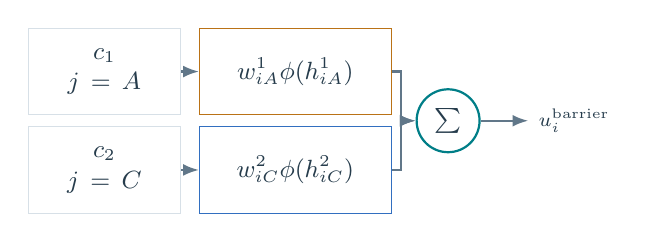
\begin{tikzpicture}[x=.97cm,y=1cm]
 \node[stage,text width=17mm](p1)at(0,0){$c_1$\\$j=A$};
 \node[stage,text width=17mm](p2)at(0,-1.25){$c_2$\\$j=C$};
 \node[stage,text width=22mm,draw=Amber](t1)at(2.5,0){$w_{iA}^{1}\phi(h_{iA}^{1})$};
 \node[stage,text width=22mm,draw=Blue](t2)at(2.5,-1.25){$w_{iC}^{2}\phi(h_{iC}^{2})$};
 \node[circle,draw=Teal,thick](sum)at(4.5,-.625){$\sum$};
 \draw[arr](p1)--(t1);\draw[arr](p2)--(t2);
 \draw[arr](t1.east)--++(.12,0)|-(sum.west);\draw[arr](t2.east)--++(.12,0)|-(sum.west);
 \draw[arr](sum)--(5.55,-.625)node[right,font=\scriptsize]{$u_i^{\rm barrier}$};
\end{tikzpicture}\par
\column{.43\textwidth}
\small
\bi{$\mathcal C_i$: relevant conflict points.\\$\mathcal N_i^m$: conflicting vehicles at $c_m$.}{$\mathcal C_i$：相关冲突点集合。\\$\mathcal N_i^m$：在 $c_m$ 处的冲突车辆集合。}
\gap
\bi{The order determines who yields. In the example, the first vehicle has zero correction weight.}{由通行顺序确定让行车辆。算例中先行车的修正权重为零。}
\end{columns}
\vspace{3mm}
\srcnote{For acceleration input: $[u]=\mathrm{m/s^2}$, $[\phi]=\mathrm{s^{-1}}$; $w$ includes an $\mathrm{m/s}$ gain. The sum is the draft's symmetric-margin form; order-aware use must retain the selected precedence.}{若控制输入为加速度：$[u]=\mathrm{m/s^2}$、$[\phi]=\mathrm{s^{-1}}$，则 $w$ 包含单位为 $\mathrm{m/s}$ 的增益。此求和式采用原文对称裕度；有序形式需保持选定的先后关系。}
\end{frame}

% 08 -----------------------------------------------------------------
\begin{frame}[t]{\bi{Worked example: prediction and correction}{计算示例：从到达预测到控制修正}}
\begin{columns}[T,onlytextwidth]
\column{.40\textwidth}
\sect{1. Observe and predict}{1. 观测并预测}
\renewcommand{\arraystretch}{1.4}
\begin{tabular}{@{}lrrr@{}}\toprule
 & $d\,(\mathrm m)$ & $v\,(\mathrm{m/s})$ & $T\,(\mathrm s)$\\\midrule
\textcolor{Teal}{$A$}&30&10&3\\
\textcolor{Amber}{$B$}&50&10&5\\\bottomrule
\end{tabular}
\gap
\[A\prec B\]
\small
\[T_{\mathrm{safe}}=1.5\,\mathrm s,\quad h_{\mathrm{act}}=1\,\mathrm s\]
\srcnote{Illustrative parameters; not calibrated settings.}{均为示意参数，并非已标定配置。}
\column{.56\textwidth}
\sect{2. Evaluate the margin}{2. 计算裕度并判断激活}
\[h=5-3-1.5=\textcolor{Amber}{0.5\,\mathrm s}<h_{\mathrm{act}}\]
\sect{3. Apply correction to the later vehicle}{3. 对后行车辆施加修正}
\[\phi=-\frac1{0.5}=-2\,\mathrm{s^{-1}}\]
\small\bi{Assume $u^{\rm headway}=0$, $w_A=0$, $w_B=0.5\,\mathrm{m/s}$.}{假设 $u^{\rm headway}=0$，$w_A=0$，$w_B=0.5\,\mathrm{m/s}$。}
\[\boxed{u_A=0,\qquad u_B=-1\,\mathrm{m/s^2}}\]
\end{columns}
\end{frame}

% 09 -----------------------------------------------------------------
\begin{frame}[t]{\bi{One feedback step increases the predicted margin}{执行一步后，重新计算预测裕度}}
\centering
\begin{tikzpicture}[x=1cm,y=1cm]
 \foreach \x/\n in {0/1,4.8/2,9.6/3}{\node[circle,fill=Teal,text=white,font=\small]at(\x+.2,.2){\n};}
 \node[anchor=west,font=\bfseries]at(.65,.2){\bi{Predict}{预测}};
 \node[anchor=west,font=\bfseries]at(5.45,.2){\bi{Brake $B$}{让 $B$ 减速}};
 \node[anchor=west,font=\bfseries]at(10.25,.2){\bi{Recompute}{重算}};
 \draw[Rule](4.35,.45)--(4.35,-2.2);\draw[Rule](9.15,.45)--(9.15,-2.2);
 \node[align=left,anchor=north west,font=\small]at(0,-.45){$T_A=3\,\mathrm s$\\[5pt]$T_B=5\,\mathrm s$\\[7pt]\textcolor{Amber}{$h=0.50\,\mathrm s$}};
 \node[align=left,anchor=north west,font=\small]at(4.8,-.45){$\Delta t=0.1\,\mathrm s$\\[5pt]$u_A=0$\\[5pt]$u_B=-1\,\mathrm{m/s^2}$};
 \node[align=left,anchor=north west,font=\small]at(9.6,-.45){$T_A^+=2.9\,\mathrm s$\\[5pt]$T_B^+=4.95\,\mathrm s$\\[7pt]\textcolor{Teal}{$h^+=0.55\,\mathrm s$}};
 \draw[arr](3.45,-.95)--(4.05,-.95);\draw[arr](8.25,-.95)--(8.85,-.95);
\end{tikzpicture}\par
\vspace{1mm}
\[d^+=d-v\Delta t-\tfrac12u\Delta t^2,\qquad v^+=v+u\Delta t\]
\small
\[\begin{array}{c|ccc}
 &d^+\ (\mathrm m)&v^+\ (\mathrm{m/s})&T^+\ (\mathrm s)\\\hline
 A&29&10&2.9\\ B&49.005&9.9&4.95
\end{array}\qquad h^+=4.95-2.9-1.5\]
\srcnote{Constant acceleration within this sample. The correction remains active; one improved prediction is not a safety proof.}{采样周期内保持加速度不变。修正仍处于激活状态；单步预测改善不构成安全性证明。}
\end{frame}

% 10 -----------------------------------------------------------------
\begin{frame}[t]{\bi{Boundaries of the original expression}{原始表达式的适用边界}}
\begin{columns}[T,onlytextwidth]
\column{.48\textwidth}
\sect{Formula and actuation}{公式与执行}
\small
\begin{itemize}\setlength\itemsep{2mm}
 \item \bi{$h=0$: undefined. $h<0$: sign reversal.}{$h=0$：无定义；$h<0$：符号反转。}
 \item \bi{A speed floor prevents division by zero, but does not validate stopped-vehicle predictions.}{速度下限避免除零，但不能保证停车车辆的预测有效。}
 \item \bi{Input limits and switching can alter the intended response.}{输入限幅与控制切换会改变预期修正效果。}
\end{itemize}
\column{.48\textwidth}
\sect{Geometry and candidate selection}{车辆几何与候选选择}
\begin{tikzpicture}[x=1cm,y=1cm]
 \fill[Road](0,0)rectangle(5.6,.6);
 \fill[Red!15](2.1,0)rectangle(3.4,.6);
 \filldraw[fill=Amber,draw=white,rounded corners=.04cm](2.8,.12)rectangle(4,.48);
 \draw[arr](4.1,.3)--(5.25,.3);
 \draw[Red,dashed](3.4,-.1)--(3.4,1.1);
 \node[tag]at(2.75,1.25){\bi{Conflict region}{冲突区域}};
 \draw[Muted](2.8,.05)--(2.8,-.4);
 \node[font=\scriptsize,anchor=north]at(2.8,-.4){\bi{Rear still inside}{车尾尚未驶离}};
\end{tikzpicture}\par
\small\bi{Point arrival times omit finite occupancy. Keeping only lane leaders also needs verification.}{点到达时间未表达完整占用过程；仅保留队首车辆的简化也需要验证。}
\end{columns}
\vspace{3mm}
\lead{Later direction: a CBF-QP safety filter}{后续方向：CBF-QP 安全过滤器}
\srcnote{The draft proposes optimization-based filtering. Feasibility, input bounds, and model assumptions must be analyzed before safety claims.}{原稿提出基于优化的过滤方案。安全结论仍需分析可行性、输入边界和模型假设。}
\end{frame}

% 11 -----------------------------------------------------------------
\begin{frame}[t]{\bi{Case A: three directed lanes, two crossing conflicts}{Case A：三条有向车道与两组交叉冲突}}
\begin{columns}[T,onlytextwidth]
\column{.49\textwidth}\centering
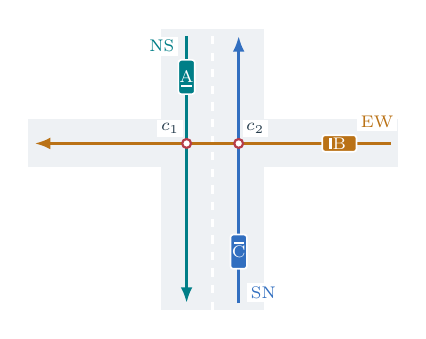
\begin{tikzpicture}[scale=.87,transform shape]
 \roadbase{1}\conflicts{1}
 \car{-.38}{1.35}{Teal}{-90}{A}
 \car{.38}{-1.2}{Blue}{90}{C}
 \car{1.85}{.38}{Amber}{180}{B}
\end{tikzpicture}\par
\srcnote{Bidirectional NS/SN; unidirectional EW.}{NS/SN 为双向道路，EW 为单向道路。}
\column{.47\textwidth}\centering
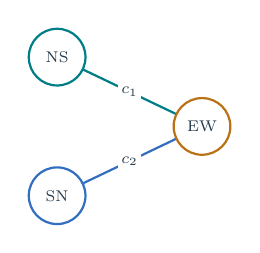
\begin{tikzpicture}[scale=.8,transform shape]\graphA\end{tikzpicture}\par
\small
\[\begin{array}{c|ccc}&\mathrm{NS}&\mathrm{SN}&\mathrm{EW}\\\hline
\mathrm{NS}&0&0&1\\\mathrm{SN}&0&0&1\\\mathrm{EW}&1&1&0\end{array}\]
\end{columns}
\vspace{1mm}
\srcnote{Separated, straight lanes. NS and SN have no crossing-conflict edge; same-lane following is handled by the nominal layer.}{假设车道分离且车辆直行。NS 与 SN 无交叉冲突边，同车道跟驰由名义控制层处理。}
\end{frame}

% 12 -----------------------------------------------------------------
\begin{frame}[t]{\bi{Case A: the EW vehicle checks both points}{Case A：EW 车辆分别检查两处冲突}}
\begin{columns}[T,onlytextwidth]
\column{.48\textwidth}
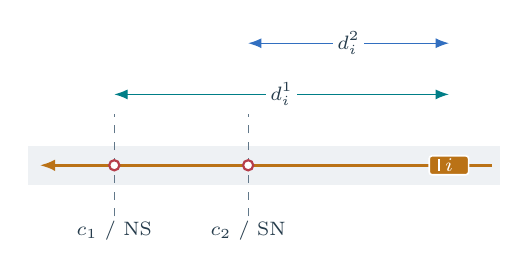
\begin{tikzpicture}[x=1cm,y=1cm]
 \fill[Road](0,0)rectangle(6,.5);
 \draw[lane,Amber](5.9,.25)--(.15,.25);
 \car{5.35}{.25}{Amber}{180}{$i$}
 \foreach \x/\c/\lane in {1.1/1/NS,2.8/2/SN}{
 \draw[Muted,dashed](\x,-.4)--(\x,.9);
 \node[dot]at(\x,.25){};
 \node[tag,anchor=north]at(\x,-.4){$c_{\c}$ / \lane};}
 \draw[<->,Teal](1.1,1.15)--node[tag]{$d_i^1$}(5.35,1.15);
 \draw[<->,Blue](2.8,1.8)--node[tag]{$d_i^2$}(5.35,1.8);
\end{tikzpicture}\par
\small\bi{Use a separate path distance and arrival prediction for each point.}{每个冲突点分别使用沿路径距离与到达时间预测。}
\column{.48\textwidth}
\sect{Pairwise correction, then aggregation}{先计算车辆对修正，再聚合}
\small
\[u_{\mathrm{EW}}^{\rm barrier}=u_{\mathrm{EW,NS}}^{\rm barrier}+u_{\mathrm{EW,SN}}^{\rm barrier}\]
\bi{Each term includes activation and the selected yielding role.}{每项修正均包含激活判断及已选定的让行角色。}
\gap
\srcnote{Priorities at the two points must be consistent; the draft leaves this coordination rule open.}{两处冲突点的优先级应保持一致；原稿尚未确定具体协调规则。}
\end{columns}
\vspace{2mm}
\hrule height .4pt\vspace{2mm}
\small\bi{Signed braking example}{带符号的制动修正示例}\quad $(-1,-3)\ \mathrm{m/s^2}$
\[
\underbrace{-1+(-3)=-4}_{\text{\bi{sum}{求和}}}\qquad
\underbrace{\min(-1,-3)=-3}_{\text{\bi{strongest individual braking}{最强单项制动}}}
\]
\srcnote{$\max(-1,-3)=-1$ gives weaker braking. Aggregation alone does not enforce actuator limits or prove safety.}{$\max(-1,-3)=-1$ 对应较弱制动。聚合运算本身不保证满足执行器限幅或安全要求。}
\end{frame}

% 13 -----------------------------------------------------------------
\begin{frame}[t]{\bi{Case B: four directed lanes and a conflict matrix}{Case B：四条有向车道与冲突矩阵}}
\begin{columns}[T,onlytextwidth]
\column{.38\textwidth}\centering
\sect{Road geometry}{道路几何}
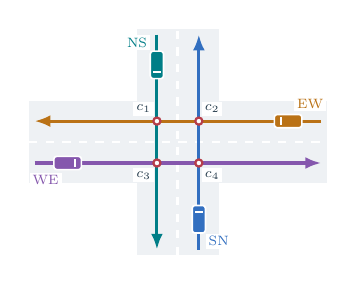
\begin{tikzpicture}[scale=.70,transform shape]
 \roadbase{2}\conflicts{2}
 \car{-.38}{1.4}{Teal}{-90}{}
 \car{.38}{-1.4}{Blue}{90}{}
 \car{2}{.38}{Amber}{180}{}
 \car{-2}{-.38}{Purple}{0}{}
\end{tikzpicture}\par
\column{.25\textwidth}\centering
\sect{Conflict graph}{冲突图}
\vspace{5mm}
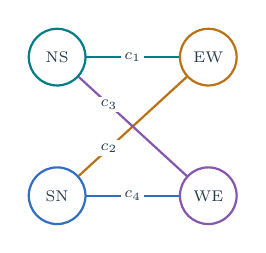
\begin{tikzpicture}[scale=.8,transform shape]\graphB\end{tikzpicture}\par
\column{.33\textwidth}\centering
\sect{Matrix $A$}{矩阵 $A$}
\vspace{3mm}
\small
\[\begin{bmatrix}0&0&1&1\\0&0&1&1\\1&1&0&0\\1&1&0&0\end{bmatrix}\]
\srcnote{Row/column order:\\NS, SN, EW, WE}{行列顺序：\\NS、SN、EW、WE}
\end{columns}
\vspace{4mm}
\lead{Four unique edges; each appears twice in the symmetric matrix}{共有四条唯一冲突边，对称矩阵中每条边出现两次}
\srcnote{c1: NS--EW; c2: SN--EW; c3: NS--WE; c4: SN--WE. Turning movements require a new conflict map.}{c1：NS--EW；c2：SN--EW；c3：NS--WE；c4：SN--WE。加入转向通行后需重新建立冲突图。}
\end{frame}

% 14 -----------------------------------------------------------------
\begin{frame}[t]{\bi{Case B: candidate selection and online calculation}{Case B：候选车选择与在线计算}}
\begin{columns}[T,onlytextwidth]
\column{.45\textwidth}\centering
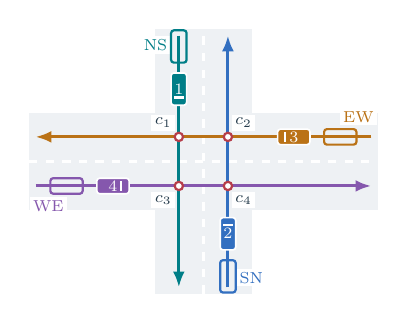
\begin{tikzpicture}[scale=.82,transform shape]
 \roadbase{2}\conflicts{2}
 \car{-.38}{1.12}{Teal}{-90}{1}\ghostcar{-.38}{1.78}{Teal}{-90}
 \car{.38}{-1.12}{Blue}{90}{2}\ghostcar{.38}{-1.78}{Blue}{90}
 \car{1.4}{.38}{Amber}{180}{3}\ghostcar{2.12}{.38}{Amber}{180}
 \car{-1.4}{-.38}{Purple}{0}{4}\ghostcar{-2.12}{-.38}{Purple}{0}
\end{tikzpicture}\par
\srcnote{Filled: leader candidate. Outline: following vehicle.}{实心：队首候选车；空心：后续车辆。}
\column{.51\textwidth}
\small
\begin{enumerate}\setlength\itemsep{2.5mm}
 \item \bi{Select the nearest approaching vehicle on each nonempty lane.}{从每条非空车道选出最近的接近车辆。}
 \item \bi{Use $A$ to select $(1,3),(2,3),(1,4),(2,4)$.}{根据 $A$ 选出 $(1,3),(2,3),(1,4),(2,4)$。}
 \item \bi{Predict arrivals, choose order, compute $h$, and test activation.}{预测到达时间，确定顺序，计算 $h$ 并判断激活。}
 \item \bi{Aggregate per vehicle, execute, then update the candidates.}{逐车聚合修正、执行控制，再更新候选车。}
\end{enumerate}
\end{columns}
\vspace{3mm}
\srcnote{Implementation requirement beyond the leader-only rule: retain occupying vehicles until rear clearance; validate that candidate reduction omits no relevant conflicts.}{队首规则之外的实现要求：区域占用车辆须保留至车尾驶离，并验证候选筛选未遗漏相关冲突。}
\end{frame}

% 15 -----------------------------------------------------------------
\begin{frame}[t]{\bi{Five experimental stages}{从单路口到路网的五阶段实验}}
\centering
\begin{tikzpicture}[x=1cm,y=1cm]
 \foreach \x/\n in {1.3/1,4.1/2,6.9/3,9.7/4,12.5/5}{\node[text=Teal,font=\large\bfseries]at(\x,1.3){S\n};}
 \begin{scope}[shift={(1.3,0)}]\draw[Navy,line width=2pt,domain=0:360,samples=100,smooth,variable=\a]plot({.9*sin(\a)},{.65*sin(2*\a)});\node[dot]at(0,0){};\end{scope}
 \begin{scope}[shift={(4.1,0)}]
 \draw[lane,Teal](-.2,.85)--(-.2,-.85);\draw[lane,Blue](.2,-.85)--(.2,.85);\draw[lane,Amber](1,0)--(-1,0);\end{scope}
 \begin{scope}[shift={(6.9,0)}]
 \draw[lane,Teal](-.2,.85)--(-.2,-.85);\draw[lane,Blue](.2,-.85)--(.2,.85);\draw[lane,Amber](1,.2)--(-1,.2);\draw[lane,Purple](-1,-.2)--(1,-.2);\end{scope}
 \begin{scope}[shift={(9.7,0)}]
 \draw[Navy,thick](-1.1,0)--(1.1,0);\foreach \x in {-.6,.6}{\draw[Navy,thick](\x,-.7)--(\x,.7);\node[dot]at(\x,0){};}\end{scope}
 \begin{scope}[shift={(12.5,0)}]
 \foreach \x in {-.8,0,.8}{\draw[Navy,thick](\x,-.6)--(\x,.6);}
 \foreach \y in {-.6,.6}{\draw[Navy,thick](-.8,\y)--(.8,\y);\foreach \x in {-.8,0,.8}{\fill[Teal](\x,\y)circle(.065);}}\end{scope}
 \foreach \x in {2.6,5.4,8.2,11}{\draw[arr](\x-.15,0)--(\x+.15,0);}
 \node[align=center,text width=2.45cm,font=\small]at(1.3,-1.5){\bi{Figure-eight\\closed loop}{八字闭环\\参考场景}};
 \node[align=center,text width=2.45cm,font=\small]at(4.1,-1.5){\bi{Open-road\\Case A}{开放道路\\Case A}};
 \node[align=center,text width=2.45cm,font=\small]at(6.9,-1.5){\bi{Open-road\\Case B}{开放道路\\Case B}};
 \node[align=center,text width=2.45cm,font=\small]at(9.7,-1.5){\bi{Two-intersection\\corridor}{双路口\\走廊}};
 \node[align=center,text width=2.45cm,font=\small]at(12.5,-1.5){\bi{Multi-intersection\\network}{多路口\\网络}};
 \node[align=center,text width=2.45cm,font=\scriptsize,text=Muted]at(1.3,-2.55){\bi{Reproduce\\reference}{复现参考行为}};
 \node[align=center,text width=2.45cm,font=\scriptsize,text=Muted]at(4.1,-2.55){\bi{Open arrivals}{开放交通流到达}};
 \node[align=center,text width=2.45cm,font=\scriptsize,text=Muted]at(6.9,-2.55){\bi{Multiple conflicts}{多方向冲突}};
 \node[align=center,text width=2.45cm,font=\scriptsize,text=Muted]at(9.7,-2.55){\bi{Downstream capacity}{下游容量约束}};
 \node[align=center,text width=2.45cm,font=\scriptsize,text=Muted]at(12.5,-2.55){\bi{Routes and scale}{路径需求与规模}};
\end{tikzpicture}\par
\vspace{3mm}
\srcnote{Proposed test sequence. Each stage expands the interaction structure; no experimental outcome is assumed.}{未来测试路线：逐步扩展交通交互结构，各阶段均不预设实验结果。}
\end{frame}

% 16 -----------------------------------------------------------------
\begin{frame}[t]{\bi{Open-road single-intersection tests}{开放道路单路口：测试输入与观测逻辑}}
\begin{columns}[T,onlytextwidth]
\column{.49\textwidth}
\sect{Matched arrivals for S2 and S3}{S2 与 S3 的配对到达输入}
\begin{tikzpicture}[x=1cm,y=1cm]
 \draw[arr](.6,0)--(6,0)node[right,font=\scriptsize]{$t$};
 \draw[arr](.6,-1.2)--(6,-1.2)node[right,font=\scriptsize]{$t$};
 \node[anchor=west,font=\scriptsize]at(.6,.65){\bi{Random arrivals}{随机到达}};
 \node[anchor=west,font=\scriptsize]at(.6,-.55){\bi{Burst / near-simultaneous}{突发或近同时到达}};
 \foreach \x in {1,1.8,3.1,3.5,5.3}{\fill[Teal](\x,0)circle(.07);}
 \foreach \x in {1.5,1.7,1.9,2.1,4.6,4.8}{\fill[Amber](\x,-1.2)circle(.07);}
\end{tikzpicture}\par
\small\bi{S2: three incoming directions.\\S3: four incoming directions.}{S2：三个驶入方向。\\S3：四个驶入方向。}
\gap
\srcnote{Use the same arrival and route files for each controller.}{不同控制器读取相同的到达与路径文件。}
\column{.47\textwidth}
\sect{Sweep demand and stress the controller}{改变需求并施加压力场景}
\small
\begin{itemize}\setlength\itemsep{2mm}
 \item \bi{Balanced flows, then one dominant approach.}{先测试均衡流量，再测试单进口占优。}
 \item \bi{Near ties, bursts, and low-speed queues.}{覆盖近同时到达、突发流与低速排队。}
 \item \bi{Observe margins, physical conflicts, delay, stops, and remaining queues.}{观测裕度、实际冲突、延误、停车与残余队列。}
\end{itemize}
\end{columns}
\vspace{3mm}
\srcnote{Use paired random seeds and report variability. Count requested, admitted, and completed vehicles, including uninserted and unfinished demand.}{采用配对随机种子并报告结果波动；统计请求进入、已进入与已完成车辆，保留未入网和未完成需求。}
\end{frame}

% 17 -----------------------------------------------------------------
\begin{frame}[t]{\bi{Corridor and network tests}{走廊与路网：从局部冲突到跨路口影响}}
\begin{columns}[T,onlytextwidth]
\column{.49\textwidth}
\sect{S4: finite storage between two junctions}{S4：路口之间的有限排队空间}
\begin{tikzpicture}[x=1cm,y=1cm]
 \fill[Road](0,-.35)rectangle(6,.35);
 \foreach \x in {.8,5.2}{\fill[Road](\x-.35,-1)rectangle(\x+.35,1);\node[tag]at(\x,1.25){$J_{\ifdim\x pt<2pt1\else2\fi}$};}
 \draw[lane,Teal](.1,-.18)--(5.9,-.18);
 \car{4.5}{-.18}{Amber}{0}{}\car{3.85}{-.18}{Amber}{0}{}\car{3.2}{-.18}{Amber}{0}{}
 \draw[Red,dashed,-{Latex}](4.7,.65)--(1.3,.65);
 \node[tag,text=Red]at(3,.95){\bi{Queue spillback}{排队向上游溢出}};
 \draw[<->,Muted](1.2,-.85)--node[tag]{\bi{Link storage}{连接路段容量}}(4.8,-.85);
\end{tikzpicture}\par
\small\bi{Track platoon discharge, travel time, and downstream queues. Can local decisions respect downstream capacity?}{跟踪车队驶出、路段行驶时间与下游排队，检验局部决策能否满足下游容量约束。}
\column{.47\textwidth}
\sect{S5: routes across a network}{S5：跨越多个路口的路径}
\begin{tikzpicture}[x=1cm,y=1cm]
 \foreach \x in {0,2,4}{\draw[Rule,line width=5pt](\x,0)--(\x,1.5);}
 \foreach \y in {0,1.5}{\draw[Rule,line width=5pt](0,\y)--(4,\y);}
 \draw[lane,Teal](-.5,0)--(2,0)--(2,1.5)--(4.6,1.5);
 \draw[lane,Amber](-.5,1.5)--(0,1.5)--(0,0)--(4.6,0);
 \foreach \x in {0,2,4}{\foreach \y in {0,1.5}{\fill[Navy](\x,\y)circle(.10);}}
 \node[tag,text=Teal]at(3,1.95){\bi{Route 1}{路径 1}};
 \node[tag,text=Amber]at(3,-.45){\bi{Route 2}{路径 2}};
\end{tikzpicture}\par
\small\bi{Increase network size, demand, and active conflicts. Measure trip delay, queues, deadlock, and computation time.}{扩大路网、增加需求与活跃冲突，测量行程延误、排队、死锁与计算耗时。}
\end{columns}
\vspace{2mm}
\srcnote{Downstream admission and inter-junction coordination are future design tasks, not existing controller capabilities.}{下游准入与跨路口协调是后续设计任务，尚非当前控制器已实现的能力。}
\end{frame}

% 18 -----------------------------------------------------------------
\begin{frame}[t]{\bi{Baselines and key performance indicators}{候选基线与关键性能指标}}
\begin{columns}[T,onlytextwidth]
\column{.43\textwidth}
\sect{Comparison methods}{对照方法}
\small
\begin{itemize}\setlength\itemsep{1.7mm}
 \item \bi{Fully actuated signal control (FAS).}{全感应式信号控制（FAS）。}
 \item \bi{Unsignalized priority control.}{无信号优先规则控制。}
 \item \bi{Original distance-difference barrier, where reproducible.}{原始距离差屏障：限可复现且适用的场景。}
\end{itemize}
\gap
\sect{Ablations}{消融配置}
\small\bi{Weighted sum / strongest signed braking / CBF-QP. Keep the same crossing-order rule where feasible.}{加权求和、最强带符号制动、CBF-QP；在可行条件下保持相同的通行顺序规则。}
\column{.54\textwidth}
\sect{Measures and units}{比较指标与单位}
\scriptsize\renewcommand{\arraystretch}{1.3}
\begin{tabular}{@{}P{.22\linewidth}P{.71\linewidth}@{}}\toprule
\bi{Efficiency}{效率}&\bi{Throughput (veh/h); mean / total delay (s/veh, s)}{吞吐量（veh/h）；平均 / 总延误（s/veh、s）}\\\midrule
\bi{Energy}{能耗}&\bi{Energy per vehicle (Wh/veh), with a specified model}{单车能耗（Wh/veh），需指定能耗模型}\\\midrule
\bi{Comfort}{舒适性}&\bi{Acceleration / jerk RMS ($\mathrm{m/s^2}$, $\mathrm{m/s^3}$); stops/veh}{加速度 / 加加速度 RMS（$\mathrm{m/s^2}$、$\mathrm{m/s^3}$）；单车停车次数}\\\midrule
\bi{Safety}{安全性}&\bi{Collisions, occupancy conflicts; minimum margin (s)}{碰撞与占用冲突次数；最小时间裕度（s）}\\\midrule
\bi{Robustness}{鲁棒性}&\bi{Deadlock count; computation time (ms)}{死锁次数；计算耗时（ms）}\\\bottomrule
\end{tabular}
\end{columns}
\vspace{2mm}
\srcnote{Match geometry, demand, vehicle limits, and seeds. Arrival-time estimate is not collision TTC. Outcomes remain to be measured.}{统一道路几何、需求、车辆约束与随机种子。预计到达时间不等于碰撞 TTC；性能结果均有待测量。}
{\fontsize{6}{7}\selectfont\color{Muted}\bi{Sources: draft, Experiments; }{来源：原稿实验章节；}\href{https://sumo.dlr.de/docs/Simulation/Traffic_Lights.html}{SUMO: traffic lights}; \href{https://sumo.dlr.de/docs/Simulation/Output/TripInfo.html}{TripInfo}; \href{https://authors.library.caltech.edu/records/jnhr0-1ww05}{Ames et al. (2017), CBF-QP}.\par}
\end{frame}
\end{document}
